\documentclass[parskip=full]{scrartcl}

\usepackage{pdfpages}
\usepackage[utf8]{inputenc}
\usepackage[T1]{fontenc}
\usepackage[german]{babel}
\usepackage{hyperref}
\hypersetup{
	pdftitle={Pflichtenheft},
	bookmarks=true,
}
\usepackage{csquotes}

\usepackage{fancyhdr}%<-------------to control headers and footers
\usepackage[a4paper,margin=1in,footskip=.25in]{geometry}
\fancyhf{}
\fancyfoot[C]{\thepage} %<----to get page number below text
\pagestyle{fancy} %<-------the page style itself

\usepackage{xcolor}
\usepackage{framed}
\definecolor{shadecolor}{RGB}{220,220,220}
\usepackage{float}


\title{Android GO! App - Pflichtenheft}
\author{Gruppe 3}
\date{11.06.17}

% define custom lists
\usepackage{enumitem}
\usepackage{lipsum}

\makeindex

\begin{document}

\begin{titlepage}
	\begin{center}
	{\scshape\LARGE \bfseries Entwurfsdokument \par}
	\vspace{1cm}
	{\scshape\Large Praktikum der Softwareentwicklung \\ Sommersemester 2017\par}
	\vspace{1.5cm}
	{\huge\bfseries Android GO! App\par}
	\vspace{2cm}
	{\Large\itshape - Gruppe 3 -\par}
	\vfill
	{\bfseries erstellt von:\par}
	Arsenii Dunaev \\
	Florian Kröger \\
	Tina Maria Strößner \\
	Volodymyr Shpylka \\	
	\vfill
	% Bottom of the page
	{\large 09.07.17 \par}	
	\end{center}
\end{titlepage}

\newpage

\begin{abstract}
Die Android App GO! ist eine mobile Applikation, die speziell zur Organisation von Treffen (z. B. gemeinsames Essen im Café oder in der Mensa) entwickelt wird. Beim erfolgreichen gemeinsamen Losgehen wird der gemittelte GPS-Standort von Mitgliedern der Gruppe angezeigt.\\

Dieses Dokument erläutert den Entwurf des Systems auf der Grundlage des Pflichtenhefts.
\end{abstract}

\newpage

\tableofcontents

\newpage

\section{Änderungen zum Pflichtenheft}

Es wurden im Entwurf folgende Änderungen gegenüber dem Pflichtenheft vorgenommen:
\begin{enumerate}
	\item \textbf{Produktdaten - Benutzer} \\
	Es werden in den Produktdaten zusätzlich eine (von Firebase automatisch generierte) InstanceID gespeichert, die es dem Server erlaubt, Daten an das Android-Gerät eines bestimmten Benutzers zu senden.
	\item \textbf{Detailansicht der GOs} \\
	Es ist jedem Mitglied einer Gruppen (unabhängig von Teilnahmestatus) möglich, die Detailansicht eines GOs aufzurufen. Um den Karten-Tab öffnen zu können, um die Standorte der anderen Teilnahmer zu verfolgen, gilt weiterhin, dass der Teilnahmestatus 'Bestätigt' oder 'Unterwegs' lauten muss.
\end{enumerate}

\newpage

\section{Architekturstil und Paketstruktur}
Dieses Kapitel erläutert den Architekturstil und die Paketstruktur des Systems. es wird noch nicht auf einzelne Klassen eingegangen sondern lediglich die Zusammenarbeit der module beschrieben und die Abhängigkeiten untereinander.

Aufgebaut ist das System mit einer Client-Server-Architektur, d.h. es gibt eine Client-Applikation, die auf den Android-Geräten der Benutzer läuft und Services des Servers in Anspruch nimmt und eine Server-Anwendung, die auf dem Tomcat-Server läuft, der diese Services bereitstellt und auf Anfrage eines Clients seine Dienste erfüllt.

\subsection{Client}
Die Architektur der Client-Applikation orientiert sich am Model-View-ViewModel (MVVM) Muster. Dies wird auf Android-Systemen durch die, auch hier eingesetzten, Architecture Components unterstützt. Das untenstehende Paketdiagramm zeigt den groben Aufbau der Client-Applikation, welche Abhängigkeiten bestehen und welche Aufgaben jedes Paket übernimmt. Genauere erläuterungen hierzu finden sich in den darauffolgenden Abschnitten.

\begin{figure}[H]
	\centering
	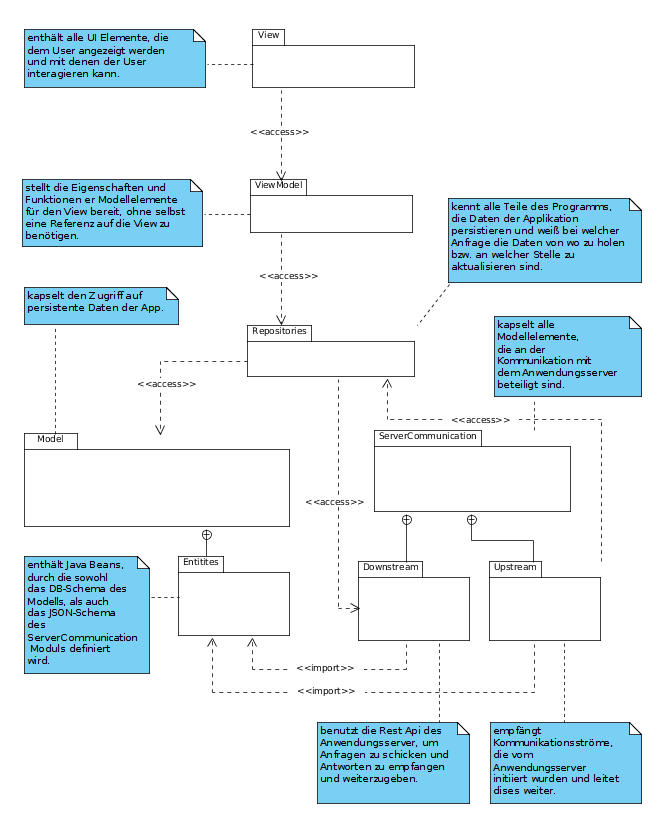
\includegraphics[scale=0.5]{../Klassendiagramme/paketdiagramm_client.png}
	\caption{Paketdiagramm der Clientanwendung}
\end{figure}

\subsubsection{Views}
Das Paket Views enthält alle Klassen, die am User Interface des Benutzers beteiligt sind. Das sind sämtliche Activities, Fragments und dazugehörige .xml-Layouts. Das Modul ist für die Präsentation der Appdaten sowie die Implementierung der Präsentationslogik (Umsetzung der Eigenschaften der Daten und Weiterleitung von Benutzereingaben) zuständig.

\textbf{Abhängigkeiten zu anderen Paketen:}\\
Das Paket Views kann die Informationen, die dem Benutzer angezeigt werden, nicht selbst generieren, sondern bekommt diese bereitgestellt von den entsprechenden ViewModells.

\textbf{Unterpakete:}\\
das Paket enthält das Unterpaket 'RecyclerView'. Da in der Applikation viele (verschiedene) RecyclerViews verwendet werden, gibt es für die Erstellung derselben ein eigenes Paket, dessen Aufgabe es ist, von den Datenobjekten die das Model liefert die gewünschten Informationen zu extrahieren und diese mit dem richtigen Layout zusammenzuführen. Innerhalb des Pakets besteht eine Abhängigkeit derjenigen View-Klassen, die einen RecyclerView verwenden zu dem Unterpaket RecyclerViews. Das Unterpaket RecyclerViews selbst ist nocht von anderen Klassen und Paketen abhängig.

\subsubsection{Modell}
Das Modell ist die Datenzugriffsschicht der Applikation, d.h. sie kapselt den Zugriff auf persistente Daten, die in einer lokalen SQLite Datenbank gehalten werden.Darüber hinaus enthält das Paket die Geschäftslogik der App, das hei?t hier werden die om ViewModel aufbereiteten und weitergeleiteten Befehle umgesetzt und anschließend die sich ergebenden Datenänderungen an das ViewModell zurückgegeben. Die Modellklassen, die sich lokal in der Applikation befinden, werden erweitert durch das Datenmodell, welches sich auf dem Server befindet. Es muss stets die Datenkonsistenz dieser zwei Modellteile sichergestellt werden (vgl. Paket Repository).

\textbf{Abhängigkeiten zu anderen Paketen}\\
Der Aufbau und die Operationen, die auf der lokalen Datenbank durchgeführt werden, werden mittels des Frameworks \textit{Room} realisiert.

\textbf{Unterpakete:}\\
Das Modell enthält das Unterpaket 'Entities'. Dies enthält die Java Entitäten, die von Room zu den Relationen der Datenbank umgesetzt werden. Die Datenbank kann von Room auch ohne eine Implementierung der Zugriffslogik aufgebaut werden. Die Entities haben demnach keine Anhängigkeiten zu anderen Klassen innerhalb des Programms. DIe Zugriffslogik der DAOs setzt hingegen die Existenz der Datenbank voraus, es gibt eine Abhängigkeit vom Modell zu den Entities.

\subsubsection{ViewModell}
Das ViewModell ist das Bindeglied zwischen View und Modell. Es tauscht Informationen mit dem Modell aus und stellt so der View öffentliche Eigenschaften und Befehle zur Verfügung, die an die Steuerungselemente der UI angebunden werden können. Dabei hat as ViewModell keine Referenz auf die View. Durch diese lose Kopplung kann die View jederzeit ausgetauscht werden, ohne dass das ViewModell verändert werden muss.

\textbf{Abhängigkeiten zu anderen Paketen}\\
Das ViewModell benötigt eine Referenz zum Modell, um die von der View empfangenen Befehle weiterleiten und die richtigen Daten von Modell anfordern zu können. Um diese Abhängigkeit zu entkoppeln und das Ansprechen der richtigen Modellkomponente zu erleichtern, wird diese Abhängigkeit über einen Vermittler ("Repository") geleitet. Dies ermöglicht das einfache Austauschen des Modells, ohne dass das ViewModell verändert werden muss.

\subsubsection{ServerCommunication}
Das Paket ServerCommunication übernimmt die Kommunikation der App mit dem Server, also das Speichern von Daten auf dem Server bzw. das Holen von Daten von dem Server. Darüber hinaus werden in diesem Paket auch Nachrichten, die vom Server gesendet werden empfangen und an das Modell zur Verarbeitung weitergeleitet.

\textbf{Abhängigkeiten zu anderen Paketen}\\
Das Paket hat keine Abhängigkeiten zu anderen Paketen der Applikation. Die Implementierung des REST-Clients erfolgt über das Framework \textit{Retrofit 2}. Hier besteht also eine Abhängigkeit zu einem externen Framework. Außerdem benötigt das Modukl zur fehlerfreien Ausführung seiner Aufgaben ein funktionierendes Backend (REST-Api, das die entsprechenden Ressourcen bereitstellt) des Systems.

\textbf{Unterpakete:}\\
Das Modul ServerCommunication setzt sich aus zwei Untermodulen zusammen. Das Modul \textit{Upstream} implementiert die Kommunikation, die über die REST-Api des Tomcat-Servers läuft, also jegliche Kommunikation, die von einem Client initiiert wird. Das Modul \textit{Downstream} hingegen ist dafür zuständig Kommunikationsströme zu empfangen, die vom Server initiiert werden und diese den Vermittlern zur Verbreitung weiterzuleiten.

\subsubsection{Repositories}
Wie in den vorherigen Abschnitten erläutert, ist die Geschäftslogik der App aufgeteilt auf den lokalen Teil (Modell) und einen Remote-Teil (ServerCommunication), die miteinander synchronisiert werden müssen. Zusätzlich müssen die ViewModells nach sämtlichen Änderungen mit den aktuellsten Daten versorgt werden. Dise Abhängigkeiten der einzelnen Komponenten werden in den Repository-Klassen zusammengefasst. Genauere Erläuterungen zur Funktionsweise finden sich in Abschnitt \ref{Vermittler}.

\textbf{Abhängigkeiten zu anderen Paketen:}\\
...

\subsection{Server}
Die Architektur ser Servers orientiert sich an einer Schichten-Architektur. Dabei handelt es sich nicht um eine klassische Schichtenarchitektur, bei der nur obere Schichten Dienste der unteren Schichten aufrufen darf. Stattdessen sind die oberen Schichten in zwei Unterpakete unterteilt. In einer Hälfte jeder Schicht gehen die Methodenaufrufe von oben nach unten, in der anderen von unten nach oben. Durch diese zwei Säulen in der Anwendung ist die Implementierung, trotz Verletzung des Schichtenmodells, leicht realisierbar, da die Unterpakete immernoch topologisch sortiebar sind, sodass
eine Implementierungsreihenfolge gefunden werden kann, bei der zu jeder Zeit die Abhängigkeiten des gerade entwickelten Moduls bereits implementiert sind.

\begin{figure}[H]
	\centering
	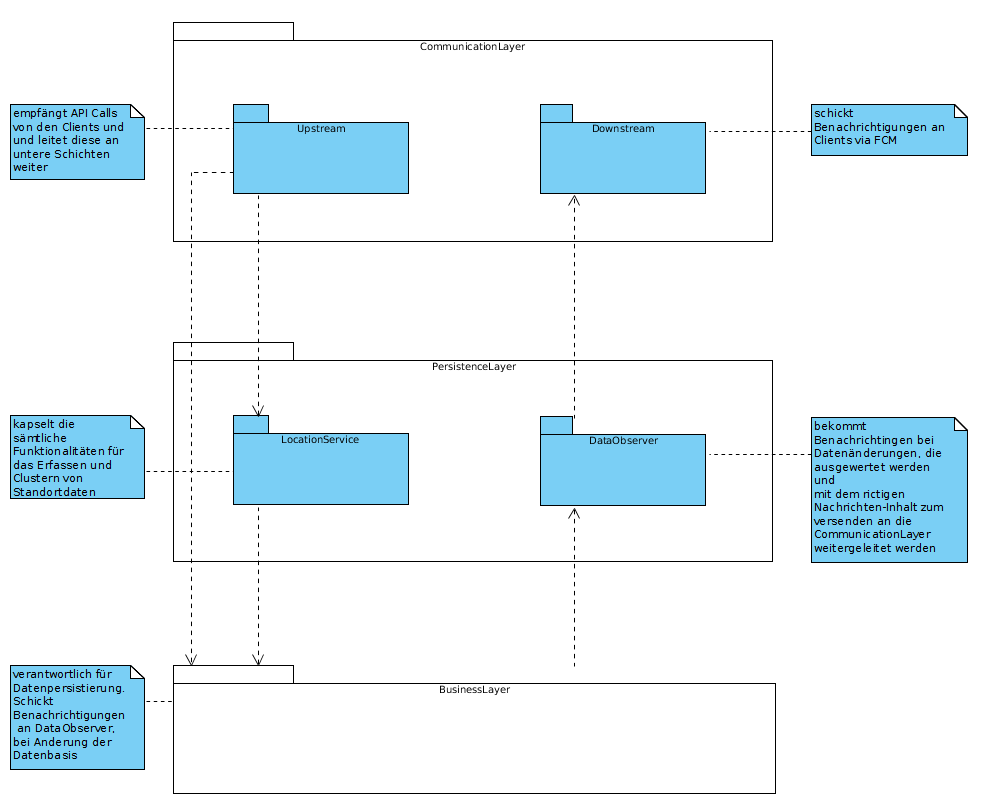
\includegraphics[scale=0.5]{../Klassendiagramme/paketdiagramm_server.png}
	\caption{Paketdiagramm der Clientanwendung}
\end{figure}

Das Programm des Servers ist in folgende Pakete aufgeteilt:
\begin{itemize}
	\item CommunicationLayer
	\item BusinessLayer
	\item PersistenceLayer
\end{itemize}

\subsubsection{CommunicationLayer}
Dieses Paket bildet die oberste Schicht der Serveranwendung und ist die einzige Schicht, die für die Clients sichtbar ist. Die CommunicationLayer vereint alle Klassen, die an der Kommunikation mit den Clients beteiligt sind. Es besteht aus den Unterpaketn Upstream und Downstream. Die Klassen des Pakets Upstream sind dafür zuständig, ein REST-API zur Verfügung zu stellen und auf Anfragen der Clients zu antworten, d.h. die Kommunikation wird von den Clients initiiert. Das Downstream-Paket hingegen schickt Nachrichten an Clients, ohne vorher von diesen angesprochen worden zu sein. Hierf"ur wird der Firebase Cloud Messaging Service benutzt.

Das Untermodul Upstream nimmt die Dineste der unteren Schichten in Anspruch. Dabei handelt es sich um eine transparente Schichtenarchitektur, das bedeutet das Modul nimmt nicht nur die Dienste der mittleren, sondern auch die Dienste der unteren Schicht in Anspruch.

Das Untermodul Downstream hingegen bietet Dienste an, nämlich das versenden von Nachrichten an Clients, die von den unteren Schichten der Serverandwendung verwendet wird.

\subsubsection{BusinessLayer}
Die BusinessLayer ist die mittlere Schicht und beinhaltet den Großteil der Anwendungslogik der Serveranwendung. Wie die anderen Schichten des Server, besteht auch die BusinessLayer aus zwei Untermodulen: LocationService und DataObserver.

Das Modul LocationService kümmert sich um alle Angelegenheiten, die mit der Erfassung, der kurzzeitigen Persistierung und dem Clustering von Standortdaten zusammenhängen. Dieser Dienst wird von der oberen Schicht in Anspruch genommen. Zur unteren Schicht bestehen keine Abhängigkeiten, da Standortdaten nicht in der datenbank gespeichert weden. Dieses Untermodul aht selbst also keine Abhängigkeiten zu anderen Paketen.

Das zweite Untermodul der BusinessLayer ist das DataObserver-Modul. Dieses Modul wird bei Anderungen in der Datenbasis von der PersistenceLayer angesprochen und kümmert sich folgend darum, die Änderungen zu analysieren, herauszufinden welche Clients von der Änderung erfahren müssen und diese Informationen an die obere Schicht weiterzuleiten, um eine Nachricht an genau diese Clients zu schicken. Dementsrechend bietet dieses Untermodul einen Dienst, der von der PersistenceLayer in Anspruch genommen wird und nimmt einen Dienst in Ansprcu der von der CommunicationLayer angeboten wird.

\subsubsection{PersistenceLayer}
Die PersistenceLayer kapselt das Datenmodellder Anwendung in sich. Sie ist für die Speicherung der Daten zuständig, sowie für die Weiterleitung der Daten an die Communicationlayer und somit an die Clients. Die PersistenceLayer setzt sich zusammen aus einer MySQL-Datenbank, die mit dem ORM-Framework Hibernate verwaltet wird und DAO-Klassen, in denen die Datenbankzugriffe gekapselt werden.

Im Gegensatz zu den zwei anderen Schichten gibt es in dieser Schicht keine Untermodule. Der Dienst des Moduls wird von dem Upstream-Modul der CommunicationLayer in Anspruch genommen. Geschieht dies, wird aus der PersistenceLayer der Dienst der DataObserver angestoßen, um die Änderungen in dem Datenbestand wieder durch die Schichten nach oben und schließlich zu den Clients zu leiten.

\newpage


\section{verwendete Entwurfsmuster}

\subsection{Schablonenmethode für SignInHelper}
Die verschiedenen Anmelde-Aktivitäten aller Loginhelper-Klassen können über die signIn()-Methode angesto"sen werden. Der spezifische Ablauf der Anmelde-Aktivität wird in den Unterklassen durch die primitiven Methoden definiert. \\

\textbf{beteiligte Klassen:}
\begin{itemize}
	\item SignInHelper: besitzt die Methode signIn(), die als Schablonenmethode dient und bei der Ausführung die primitiven Methoden configureSignIn() und startSignInProcess() aufruft
	\item FirebaseSignInHelper: Unterklasse von SignInHelper, die die primitiven Methoden configureSignIn() und startSignInProcess() implementiert
	\item GoSignInHelper: Unterklasse von SignInHelper, die die primitiven Methoden configureSignIn() und startSignInProcess() implementiert
\end{itemize}

\subsection{Beobachter zum Aktualisieren des UI}
Durch das Ausführen von Befehlen von einem Benutzer, kann es zu Änderungen in den Daten kommen, die eine Änderung des aktuellen Views anderer Benutzer erfordern. Diese 1-zu-n Abhängigkeit wird durch ein Beobachter-muster behandelt. Die dafür benötigte Funktionalität wird von der Architecture-Components Framework Klasse LiveData<> bereitgestellt. Ein Objekt dieser Klasse kann von einem LifeCycleOwner (z.B. eine Lifecycle-Activity oder ein LifecycleFragment) beobachtet werden und löst bei Änderung den Methodenaufruf \textit{onChanged()} aus. Die Livedata-Objekte sind Lifecycle-Aware, das bedeutet eine Benachrichtigung über eine Änderung wird nur dann an einen Beobachter weitergeleitet, wenn er sich in einem aktiven Stadium seines Lifecycles befindet.\\
\textbf{beteiligte Klassen:}
\begin{itemize}
	\item \textit{LiveData<>:}\\ das beobachtete Subjekt
	\item \textit{BaseActivity (die von LifecycleActivity erbt):}\\ Der Beobachter, der bei Änderung der Daten benachrichtigt wird und daraufhin das dem Benutzer präsentierte UI aktualisiert.
\end{itemize}

\subsection{Beobachter zum Weiterleiten von Änderungen der Datenbasis}
Werden von einem Client Daten der App geändret (z.B. eine GO erstellt, ein Benutzer zu einer Gruppe hinzugefügt) betrifft dies in vielen auch die Daten, die ein anderer Client bei sich gespeichert hat und benutzt. Dementsprechend müssen Clients vom Server über Änderungen in der DAtenbasis informaiert werden können. Es ergibt sich eine 1-zu-n-Abhängigkeit: n Clients sind von 1 Datenbasis abhängig.

Zur Auflösung dieser Abhängigkeit wird in der Anwendung eine Beobachter-Muster verwendet. Die Datenbasis wird beobachtet und bei Änderungen leiten die Beobachter die Benachrichtigung der Clients
ein. Da ein Beobachter nicht ein einzelnes Objekt, sondern eine gesamte Datenbanktabelle beobachet, ist es schwierig, den aktuellen Zustand des Subjekts im Beobachter zu speichern. Aus idesem Grund verwenden die beobachter eine push-Methodik, bei der die Änderungen bei der Benachrichtigung der Beobachter mit übergeben werden.

\textbf{beteiligte Klassen:}
\begin{itemize}
	\item \textit{Observable<T>}\\ Das Interface ist das abstrakte Subjekt. Jedes konkrete Subjekt muss dieses Interface und damit die Methode notify() implementieren. Diese Methode benachrichtigt die Beobachter über ein Update in der Datenbasis.
	\item \textit{DAO-Klassen}\\ Diese Klassen implementieren das Interface Observable und sind die konkreten Subjekte, die von den Beobachtern beobachtet werden.
	\item \textit{Observer}\\ Das Interface Observer ist der abstrakte Beobachter. Jeder konkrete Beobachter muss dieses Interface und damit die Methode update() implementieren.
	\item \textit{EntityObserver}\\Konkrete Beobachter, die das Interface Observer implementieren. Jede dieser Klassen übernimmt die Verantwortung für bestimmte Änderungen in der Datenbasis, analysiert, welche Änderung geschehen ist und übergibt diese Daten zum versenden an den FcmClient.
\end{itemize}

\subsection{DAO-Pattern zur Persistierung von Daten}
Die Daten der App werden in eine MySQL-Datenbank persistiert. Für den Zugriff auf diese Datenbank wird ein Data Access Object Entwurfsmuster verwendet. Dabei werden zum Einen Java Beans verwendet, die die Struktur der Datenbankrelationen festlegen. Zum Anderen gibt es spezielle DAO-Klassen die alle Datenbankzugriffe in sich kapseln. So können zusätzliche Zugriffsmethoden für die Datenbank hinzugefügt werden, ohne die Entity-Klassen verändern zu müssen. Andersherum kann der Aufbau der Datenbank verändert werden, ohne dass die DAO-klasseni ihre Schnittstelle nach außen verändern.
Die Umsetzung der Datenbank und der SQL-Queries wird mithilfe des Frameworks Hibernate realisiert.\\

\textbf{beteiligte Klassen:}
\begin{itemize}
	\item \textit{UserEntity, GoEntity, GroupEntity}\\ Entity-Beans, die die Struktur der Datenbankrelationen darstellen
	\item \textit{AbstractDAO}\\ INterface für eine DAO-Klasse, wleches Zugriffsmethoden definiert, die auf jeder Datenbanktabelle durchgeführt werden müssen (CRUD)
	\item \textit{UserDao, GoDao, GroupDao}\\ Data-Access-Object Interfaces, die spezielle Zugriffsmethoden enthalten, die nur für bestimmte Datenbanktabellen gebraucht werden.
	\item \textit{UserDaoImp, GoDapImp, GroupDaoImp}\\ konkrete IMplementierungen der DAO Interfaces. Hier werden die Zugriffsmethoden anhand des von den Entity-Klassen definierten Datenbankschemas
	implementiert.
\end{itemize}

\subsection{Vermittler zur Koordination von Datenzugriffen}\label{Vermittler}
Viele Apps Nutzen eine lokale Datenbank, um eine Benutzung der App, zumindest ansatzweise, auch ohne Internetverbindung zu ermöglichen. Auch wenn in diesem Entwurf keine lokale Datenbank auf den CLients vorgesehen ist, soll dieses Feature leicht erweiterbar sein. Zu diesem Zweck ist bei der Aktualisierung/Beschaffung der Daten für die ViewModels eine zusätzliche Indirektionsstufe eingebaut: Die Repositories. Diese übernehmen im Zusammenspiel der App-Komponenten eine Vermittler-Funktion: Während die ViewModels wissen WAS gemacht werden muss (da diese die aktuellen Daten und Funktionen für den User speichern), wissen die Repositories WO dies getan werden muss - in der lokalen Datenbank, in den SharedPreferences des Andorid-Geräts oder auf dem Remote Server.

\textbf{beteiligte Klassen:}
\begin{itemize}
	\item \textit{GoRepositor, GroupRepository, UserRepository:}\\
	 Die Vermittler die die Koordination der Kollegen übernehmen
	\item \textit{ViewModell, TomcatRestApi, lokale Datenbank, SharedPreferences:}\\ Kollegen, die nichts voneinander wissen, sondern bei allen Aufrufen vom vermittler angesprochen werden, bzw. den Vermittler ansprechen.
\end{itemize}

\subsection{Strategiemuster zur Kapselung des Clustering-Alogithmus}
Das Clustern der Standorte der Teilnehmer eines GOs wird von der Klasse GoClusterStrategy übernommen. Diese Klasse ist mittels eines Strategy-Patterns in das Programm eingebunden. Dies entkoppelt den Algorithmus von seinem Kontext und erkann dynamisch durch andere Clustering-Alogirthmen ersetzt oder ergänzt werden. \\

\textbf{beteiligte Klassen:}
\begin{itemize}
	\item \textit{LocationService} \\
	Die Klasse ist der Kontext der Clustering-Strategie. Von hier aus wird die Ausführung des Algorithmus angestoßen.
	\item \textit{ClusterStrategy} \\
	ClusterStrategy ist ein Interface, das von jedem Cluster-Algorithmus implementiert werden muss. Es definiert eine \textit{caluculateCluster()} Methode, die eine Liste an einzelnen User-Standorten entgegen nimmt und eine Liste an User-Clustern zurückgibt.
	\item \textit{GoClusterStrategy} \\
	In dieser Klasse wird der Clustering-Algorithmus implementiert, der angewendet werden soll. Die Klasse erweitert das Interface ClusterStrategy.
\end{itemize}

\subsection{Fassade zur Vereinfachung des Server Interfaces}
Der verwendete Tomcat-Server bietet seinem Clients zur Kommunikation ein REST Interface an. Das Ansprechen der verschiedenen REST Ressourcen ist in der App hinter dem Interface \textit{TomcatRestApi}. Das Interface bietet den aufrufenden Klassen Methoden zum aufrufen der REST Ressourcen an, ohne das ein Aufrufer etwas von der eigentlichen Kommunikation mit dem Server wissen muss. \\

\textbf{beteiligte Klassen}
\begin{itemize}
	\item \textit{TomcatRestApi} \\
	Das Interface ist die Fassade, die die Schnittstelle zum Tomcat-Server hinter sich versteckt. Nach außen werden Methoden bereitgestellt, die von anderen Klassen aufgerufen werden können, um Server-Dienste in Anspruch nehmen zu können, ohne sich um die Details der Kommunikation zu kümmern.
\end{itemize}

\subsection{Dekorierer zur Erweiterung der Aktivitäten für Sonderbenutzer}
Für GO-Verantwortliche und Gruppenadmins werden GroupDetailActivity oder GoDetailActivity entschprechend erweitert. Zusätzliche Buttons und Methoden werden hinzugefügt.(z.B. Name der Gruppe ändern, Mitglieder hinzufügen usw.) Dazu haben wir eine Android-Version von Dekorierer benutzt. Die spezielle Unterklassen (GroupDetailActivitzOwner bzw. GoDetailActivityOwner) von oben genannten Activities benutzen fertige Oberklassen Activities und fügen darauf die benötigte Funktionalität hinzu.

\textbf{beteiligte Klassen}
\begin{itemize}
\item \textit{GroupdetailActivity} \\
Activity, wo die Gruppendetails angezeigt werden. Ist eine Oberklasse von GroupDetailActivityOwner.
\item \textit{GroupDetailActivityOwner}
Erweitert die Oberklasse um Funktionen für die Admins.
\item \textit{GoDetailActivity}
Activity, wo Go-Details angezeigt werden. Oberklasse von GoDetailActivityOwner.
\item \textit{GoDetailActivityOwner}
Erweitert die Oberklasse um Funktionen für den GO-Verantwortlichen
\end{itemize}


\subsection{Command Muster zur Bearbeitung der Server Messages auf der Client Seite}


\newpage

\section{Client-Server-Schnittstelle}
Dieser Abschnitt erläutert die Schnittstelle zwischen dem Client und dem Server. Diese Schnittstelle besteht aus zwei Teilen:

Zum Einen bietet der Server eine REST API an, über die der Client die Dienste des Servers in Anspruch nehmen kann. Zum Anderen gibt es eine Schnittstelle, die über Firebase Cloud Messaging realisiert ist, damit der Server Nachrichten an bestimmte Clients schicken kann.

\subsection{REST API des Servers}
Folgende Grafik zeigt, welche Methoden unter welchen URL des Servers zu erreichen sind:
\begin{figure}[H]
	\centering
	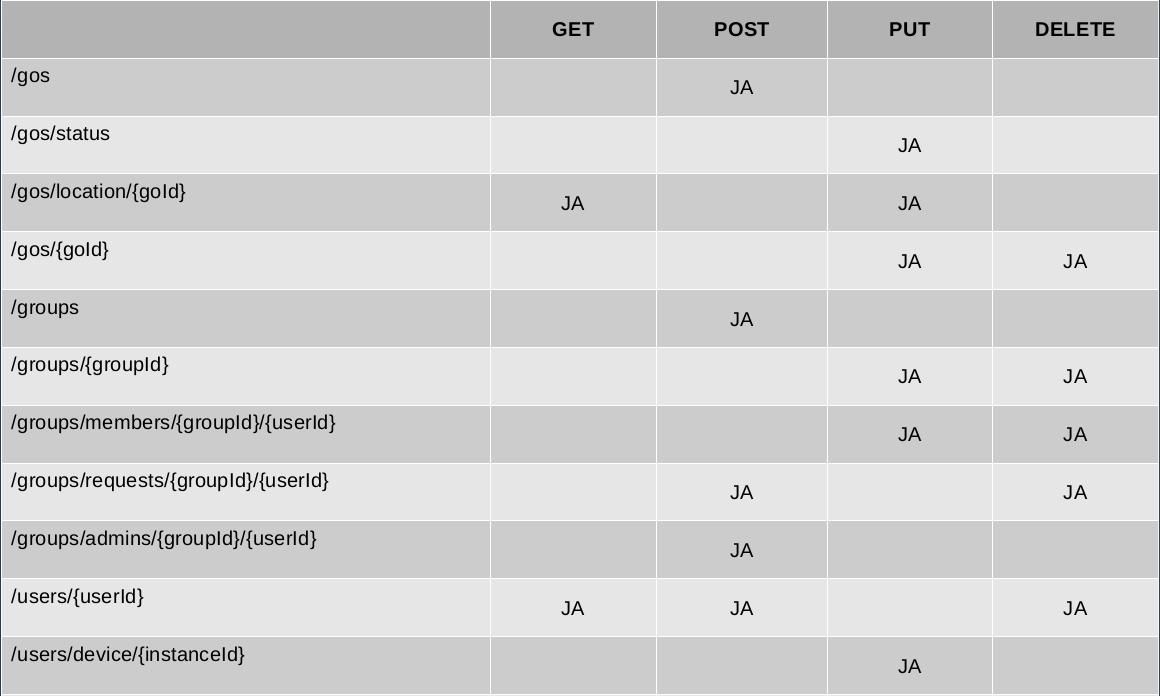
\includegraphics[width=0.8\textwidth]{restapi.png}
	\caption{Übersicht über die Rest Api des Servers}
\end{figure}
Aufrufe der Request-Methoden DELETE und GET enthalten keinen Content-Body. Sämtliche Informationen, die der Server braucht, um richtig auf die anfrage antworten zu können, sind in der URL kodiert.
Bei den Methoden POST und PUT, sowie bei Antworten des Servers, die einen Content-Body erfordern, ist sind die Daten in einem JSON-Objekt gekapselt. Dieses Objekt wird von dem Framework Gson aus der entsprechenden Entity-Klasse erzeugt. die Anwendung muss den genauen Aufbau des JSON Objekts nicht kennen. Die Verantwortung für die Verwaltung derselben wird hier vollständig an Gson übergeben.

Bei sämtlichen Requests kann der Client anhand des HTTP-Statuscodes der Server-Response erkennen, ob die Anfrage erfolgreich ausgeführt werden konnte.

\subsection{FCM Schnittstelle}
Die Schnittstelle zwischen Server und Client, die zum Senden von Downstream-Nachrichten verwenet werden kann, wird über Firease Cloud Messaging realisiert. Der Server sendet einen HTTP Post Request an den Firebase Server. Dabei besteht der Content-Body dieser HTTP-Anfrage aus einem JSON-Objekt indem der Empfänger und die zu übermittlenden Daten spezifiziert sind.

Folgende Grafik \footnote{Quelle: https://firebase.google.com/docs/cloud-messaging/send-message} zeigt den Aufbau eines HTTP-Requests, wie er an den FCM Server gesendet werden muss für eine erfolgreiche Weiterleitung der Nachricht:

\begin{figure}[H]
	\centering
	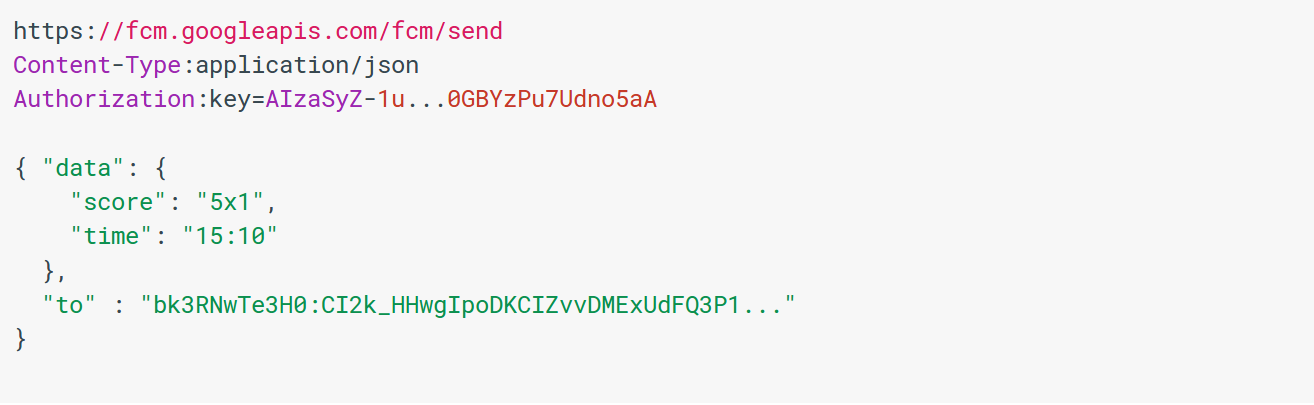
\includegraphics[width=1\textwidth]{http_format.png}
	\caption{Beispiel für ein HTTP-Request an den FCM Server}
\end{figure}

Das in grün markierte JSON-Objekt kann dabei je nach Anwendungsfall ein anderes Data-Field enthalten. Das "to"-Feld enthält die instanceId des Empfängers der Nachricht.

\textbf{Inhalt des 'data'-Felds für die verschiedenen Anwendungsfälle der App:}
Zunächst enthalten sämtliche Nachrichten unter dem Tag "tag" einen String der signalisiert, was der Anlass zum Senden der Nachricht war. Bei diesen Strings handelt es sich um Elemente des Enums EventArg.
\begin{itemize}
	\item \textit{Go Added}\\
	Ein aus einer GO-Entität erzeugtes JSON-Objekt unter dem Tag 'go'. Dieses wird automatisch durch das Framework Gson erzeugt.
	\item \textit{Go Edited}\\
	Ein aus einer GO-Entität erzeugtes JSON-Objekt unter dem Tag 'go'. Dieses wird automatisch durch das Framework Gson erzeugt. Es werden allerdings die Listen der Go-Teilnehmer aus dem Objekt entfernt,
	da Änderungen derselben von diesem Anwendungsfall nicht betroffen sind und die Daten somit nicht übertragen werden müssen.
	\item \textit{Go Removed}\\
	Die ID des entfernten Gos unter dem Tag 'id'
	\item \textit{Group Edited}\\
	Ein aus einer Group-Entität erzeugtes JSON-Objekt unter dem Tag 'group'. Dieses wird automatisch durch das Framework Gson erzeugt. Es werden allerdings die Listen der Gruppenmitgleider und Administratoren aus dem Objekt entfernt, da Änderungen derselben von diesem Anwendungsfall nicht betroffen sind und die Daten somit nicht übertragen werden müssen.
	\item \textit{Group Removed}\\
	Die ID der entfernten Gruppe unter dem Tag 'id'
	\item \textit{Group Request Received}\\
	Ein aus einer Group-Entität erzeugtes JSON-Objekt unter dem Tag 'group'. Dieses wird automatisch durch das Framework Gson erzeugt
	\item \textit{Member Added}\\
	Die ID der Gruppe zu der der Benutzer hinzugefügt werden soll unter dem Tag 'id'. Unter dem Tag 'user' ist ein JSON-Objekt gespeichert, das aus einer User-Entität erzeigt wurde. Dies geschieht automatisch durch das Framework Gson.
	\item \textit{Member Removed}\\
	Die ID des Benutzers, der aus der Gruppe entfernt werden soll unter dem Tag 'user\_id' und die ID der Gruppe, aus der der Benutzer entfernt werden soll unter dem Tag 'group\_id'.
	\item \textit{Admin Added}\\
	Die ID des Benutzers, der als Adminsitrator hinzugefügt werden soll unter dem Tag 'user\_id' und die ID der Gruppe, in der dies geschehen soll unter dem Tag 'group\_id'. Es ist nicht nötig das vollständige User-Objekt zu senden, da dies bereits auf den Clients in dem entsprechenden Gruppen-Objekt gespeichert ist.
	\item \textit{Status Changed}\\
	Die ID des Benutzers, der seinen Status geändert hat unter dem Tag 'user\_id', die ID des GOs in der die Statusänderung stattgefunden hat unter dem Tag 'go\_id' und eine Zahl, die den neuen Status repräsentiert, unter dem Tag 'status'. Es gilt '0': ABELEHNT, '1': BESTÄTIGT, '2': UNTERWEGS.
\end{itemize}

Bei den Clients kommt die gesendete Nachricht als remoteMessage-Objekt an. Durch die getData()-Methode kann auf den Content-Body, also das JSON-Objekt, das den eigentlichen Inhalte der Nachricht entält zugegriffen werden.

\section{Sequenzdiagramme}

\subsection{Hinzufügen eines Gruppenmitglieds}

\begin{figure}[H]
	\centering
	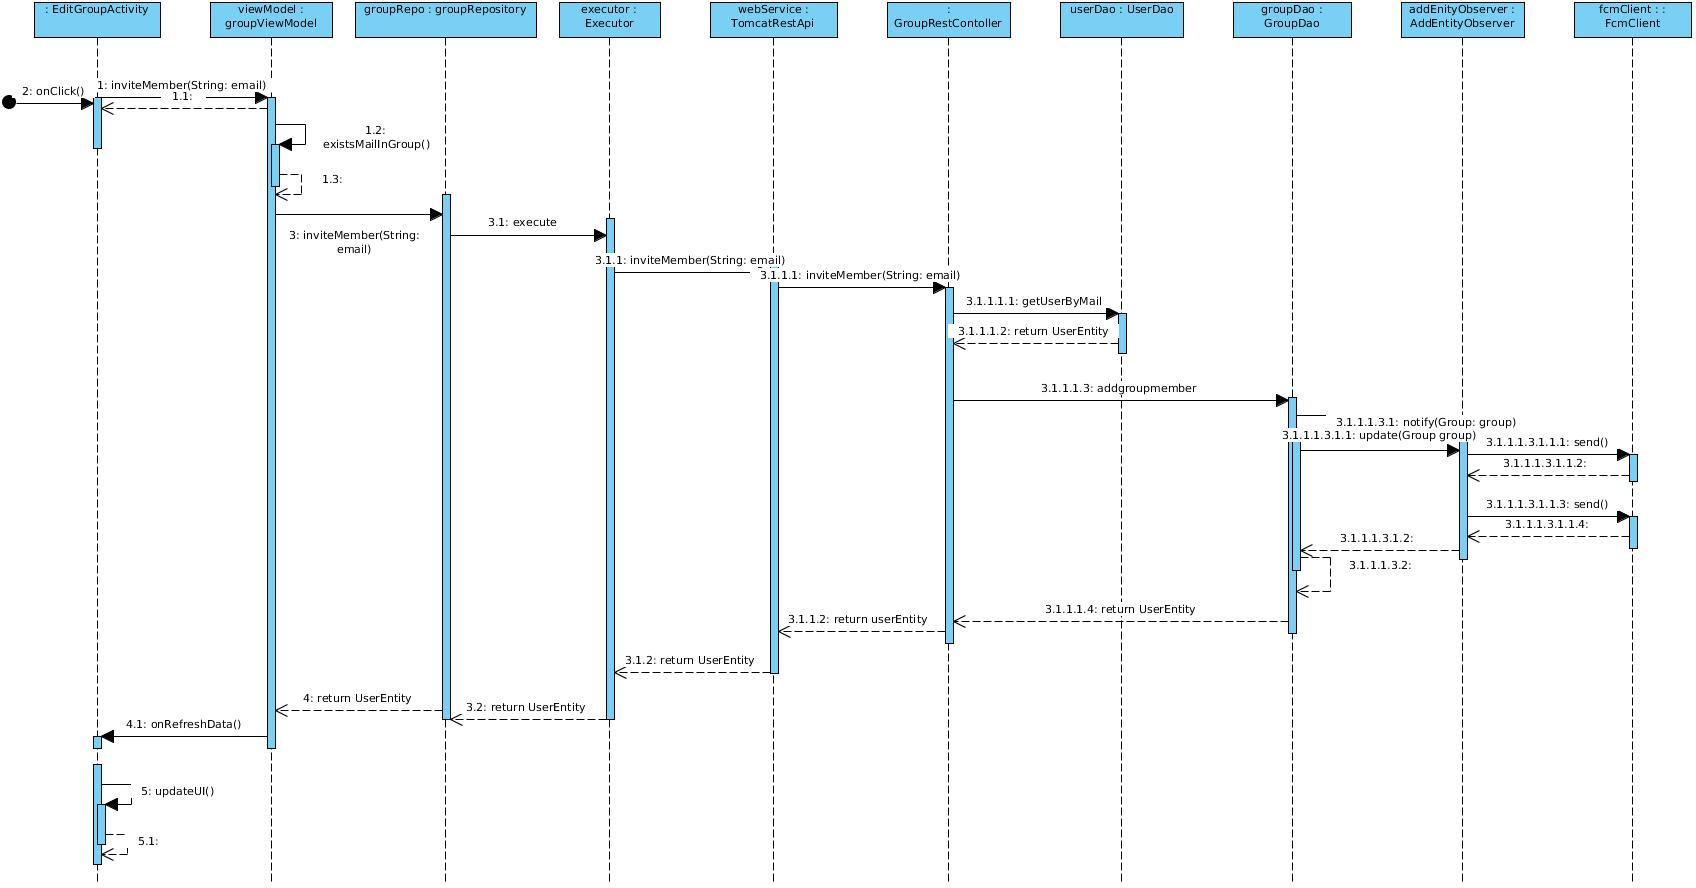
\includegraphics[width=1\textwidth]{../Sequenzdiagramme/addGroupMember.jpg}
	\caption{Sequenzdiagramm - Hinzufügen eines Gruppenmitglieds Teil 1}
\end{figure}

Das obige Sequenzdiagramm zeigt, was während der Ausführung des Programms passiert, wenn ein Benutzer die Funktion "inviteMember" ausführt. Das User Interface stellt dem Benutzer ein Textfeld zur Eingabe der E-Mailadresse und einen Button zum Bestätigen zur Verfügung. Bei Klick dieses Buttons extrahiert die Activity-Klasse die eingegebene Mail-Adresse aus dem Textfeld und übergibt diese an das ViewModel über den Methodenaufruf "inviteMember". Das ViewModel überprüft zunächst ob es bereits einen Benutzer in Gruppe gibt, der diese E-Mailadresse besitzt. Falls nicht, wird die Gruppeneinladung an die Grouprepository weitergeleitet und von dort über die Klasse TomcatrestApi an den Server gesendet.

Empfängt der Server eine Anfrage, einen User zu einer Gruppe hinzuzufügen, wird diese Anfrage zunächst an das UserDao weitergegeben. Dort wird zuerst die Methode getUserByMail() aufgerufen, um den richtigen Benutzer aus der Datenbank zu finden. Danach wird die addGroupmember-methode des GroupDaos aufgerufen. In dieser methode wird die neue gruppenanfrage in der Datenbank gespeichert und es werden die Observer benachrichtigt, dass sich Daten geändert haben.

Der AddEntityObserver erkennt, dass es sich um eine Änderung handelt, die seinen Veratnwortlichkeitsbereich betrifft. Er bekommt beim Aufruf der update()-Methode die Gruppe mit der zusätzlichen Gruppenanfrage übergeben. Der Observer extrahiert alle Gruppenmitglieder aus dem Gruppenobjekt und ruft die send()-methode des FcmClients auf, um das geänderte Gruppenobjekt an alle Gruppenmitglieder zu senden. Danach wird die send()-Methode ein zweites Mal aufgerufen, um dem neuen Gruppenmitglied die neue Gruppenanfrage zu übermitteln.

\begin{figure}[H]
	\centering
	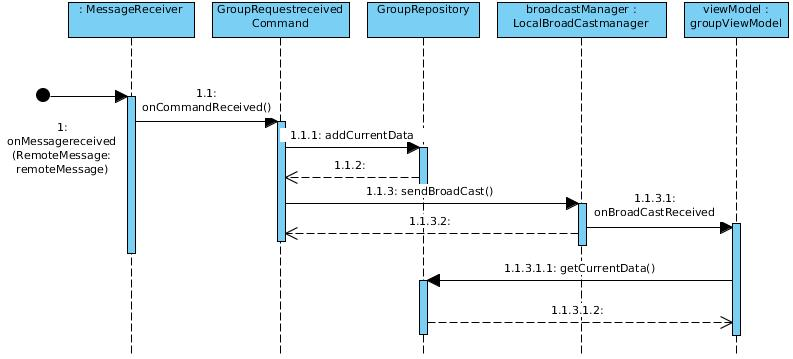
\includegraphics[width=1\textwidth]{../Sequenzdiagramme/addMember2.jpg}
	\caption{Sequenzdiagramm - Hinzufügen eines Gruppenmitglieds Teil 2}
\end{figure}

Das zweite Sequenzdiagramm zeigt, was passiert, wenn an einen Benutzer eine Gruppenmitgliedschaftsanfrage gesendet wird. Die Nachricht, die von dem Server, über dem Firebase Cloud Messaging Server, an den Client gesendet wird, löst einen Aufruf der Methode onMessageReceived() in der Klasse MessageReceiver aus. Diese Klasse extrahiert das JSON-Feld COMMAND\_CODE aus dem empfangenen JSON-Objekt und findet so heraus, an welches ServerCommand-Objekt die Anfrage weitergeleitet werden muss.

Nach Weiterleitung der Anfrage an den GroupRequestReceivedCommand wird dort das Datenfeld aus der JSON-Nachricht extrahiert. dort ist die Gruppe gespeichert, zu der er Benutzer eingeladen wurde. Diese Gruppe wird in dem öffentlichen "CurrentData" Field des GroupRepository gespeichert. Danach schickt das GroupRequestReceivedCommand-Objekt einen Broadcast an alle ViewModels. Das GroupViewModel erkennt, dass der Broadcast eine Änderung der Gruppen des Benutzers betrifft. Daher wird dort die onBroadcastReceived()-Methode auferufen. Daraufhin holt sich das ViewModel die aktualisierten Daten von der GoupRepository ab, durch einen Aufruf der getCurrentData()-Methode. Da das UI die LiveData der ViewModels beobachtet, wird automatisch bei einer Aktualisierung des ViewModels auch das UI aktualisiert und zeigt die neuen Daten an.

\subsection{Entfernen einer Gruppe}

\begin{figure}[H]
	\centering
	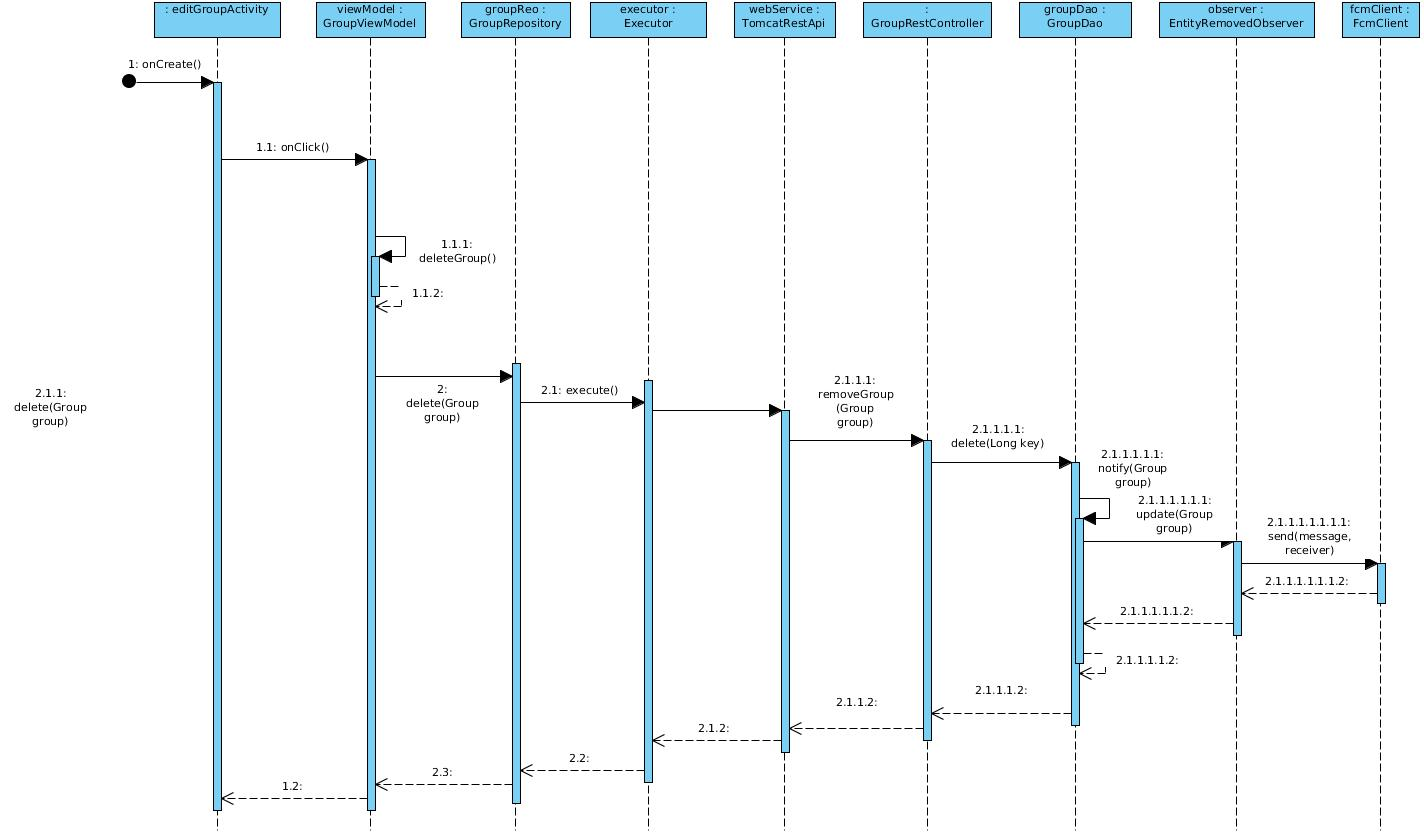
\includegraphics[width=1\textwidth]{../Sequenzdiagramme/deleteGroup_sequenz.jpg}
	\caption{Sequenzdiagramm - Entfernen einer Gruppe}
\end{figure}

Das obige Sequenzdiagramm zeigt den Programmablauf, nachdem ein Benutzer die "Gruppe löschen"-Funktion ausgelöst hat. Das UI gibt den Button Press an das GroupViewModel weiter. Dort wird die Gruppe zunächst in den lokaeln Daten gelöscht. Dabei muss sichergestellt werden, dass die Daten nach dem Löschen konsistent sind, also z.B. auch alle GOs der Gruppe gelöscht wurden.

Danahc wird die Anfrage über die GroupRepository und das Rest API an den Server übergeben, wo sie durch den Methodenaufruf deleteGroup() in der GroupRestController-Klasse ankommt. Von dort aus wird die Anfrage an das GroupDao gegeben, welches die Gruppe in der Datenbank löscht. Auch hier muss auf die Konsistenz der Daten geachtet werden. Danach werden die Observer des GroupDaos benachrichtigt, dass eine Ändeurng stattgefunden hat. Da die Änderung nur den EntityRemovedObserver betrifft, wird bei diesem Objekt die Methode update() aufgerufen. Mit dem Methodenaufruf wird auch die gelöschte Gruppe übergeben.

Der Observer baut ein Message-Objekt aus der erhaltenen Gruppe und extrahiert eine Listse aller Gruppenmitglieder aus dem Gruppenobjekt. Diese Daten werden witergegeben an dem FcmClient über die Methode send(). Dadurch werden die Nachrichten über die Löschung der Gruppe an die Gruppenmitglieder geschickt, damit diese ihre lokalen Daten anpassen können.


\end{document}

